% Document layout
\documentclass[a4paper,11pt]{article}
\usepackage[a4paper, inner=2.5cm , outer=2.5cm, top=2cm, bottom=2cm]{geometry}
\usepackage[usenames,dvipsnames]{color}
% Referencing & fonts
\usepackage[sort&compress]{natbib}
\setlength{\bibsep}{0.0pt}
\usepackage[font=small,labelfont=bf]{caption}
\usepackage[OT2,T1]{fontenc}
% Set formats for each heading level
\usepackage{sectsty}
\allsectionsfont{\usefont{OT1}{phv}{bc}{n}\selectfont}
\sectionfont{\color{MidnightBlue}}              % sets colour of sections
\subsectionfont{\color{MidnightBlue}}        % sets colour of subsections
\subsubsectionfont{\color{MidnightBlue}}  % sets colour of subsections
% Other shit
\usepackage{algorithm}
\usepackage{amsfonts}
\usepackage{amsmath}
\usepackage{amssymb}
\usepackage{bbm}
\usepackage{booktabs}
\usepackage{epsfig}
\usepackage{float}
\usepackage[font=normalsize]{caption}
\usepackage{graphicx}
\usepackage{hyperref}
\usepackage{lineno}
\usepackage{mathtools}
\usepackage{sidecap}
\usepackage{sectsty}
\usepackage{verbatim}
\usepackage{wrapfig}
\usepackage{xcolor}
\usepackage[most]{tcolorbox}
\usepackage{lipsum}
% Declarations
\DeclarePairedDelimiter\floor{\lfloor}{\rfloor}
\DeclareSymbolFont{cyrletters}{OT2}{wncyr}{m}{n}
\DeclareMathSymbol{\Sha}{\mathalpha}{cyrletters}{"58}
\DeclareMathSymbol{\sha}{\mathalpha}{cyrletters}{"57}
% Defined commands
\newcommand{\nc}{\newcommand}
\nc{\be}{\begin{equation}}
\nc{\ee}{\end{equation}}
\nc{\bea}{\begin{eqnarray}}
\nc{\eea}{\end{eqnarray}}
\newcommand{\prgname}[1]{\textcolor{NavyBlue}{\texttt{#1}}}
\newcommand{\linkfont}[1]{\textcolor{BurntOrange}{\textbf{#1}}}
\newcommand{\shellcmd}[1]{\\\indent\indent\texttt{\$ #1}}
\newcommand{\shellctd}[1]{\\\indent\indent\texttt{#1}}
\newcommand{\ra}[1]{\renewcommand{\arraystretch}{#1}}
\begin{document}
\begin{figure}
\centering
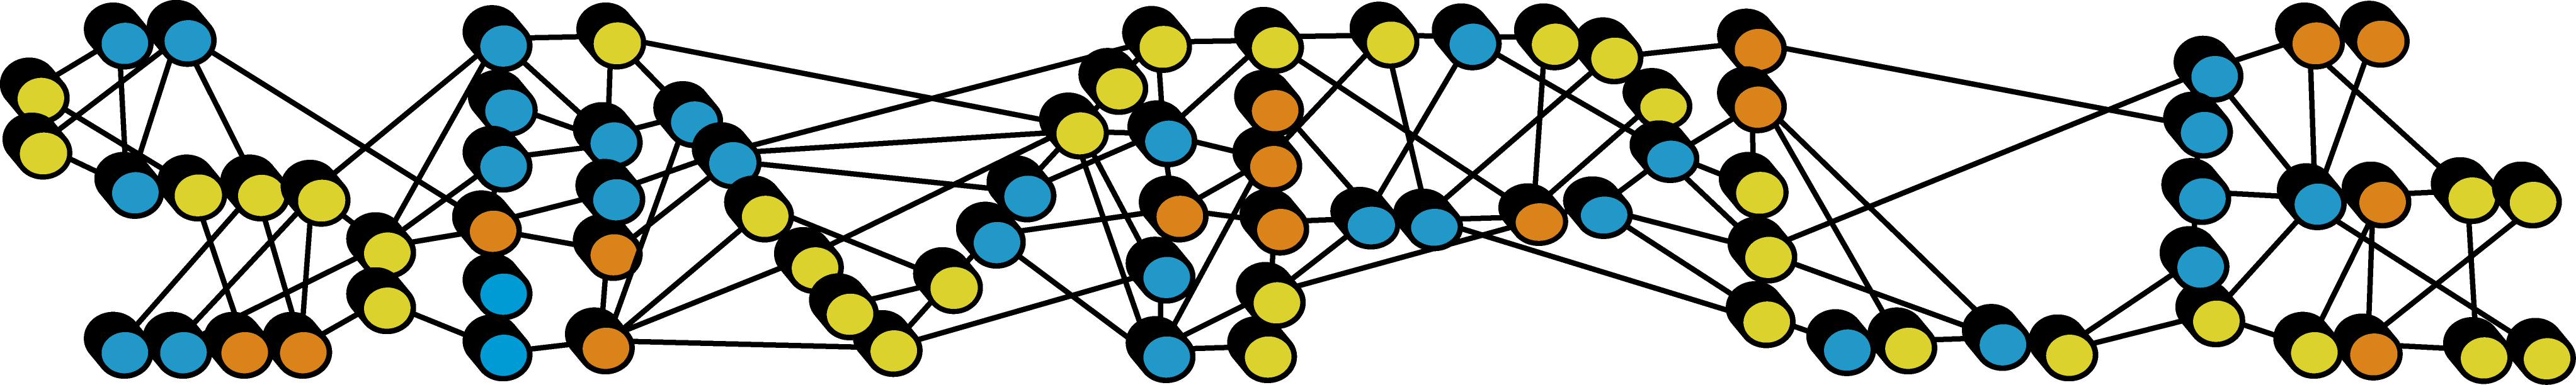
\includegraphics[keepaspectratio=true,scale=0.6]{./SIMPLE_logo/rawlogo}
%\caption{}
\end{figure}

\title{\prgname{SIMPLE Tutorial 2017}}
\author{Dominika Elmlund, Hans Elmlund}
\maketitle

\vspace{1em}
\begin{minipage}[ht]{0.48\textwidth}
\textbf{Contributors:}\\
cyril.reboul@monash.edu\\
michael.eager@monash.edu\\
dominika.elmlund@monash.edu\\
hans.elmlund@monash.edu\\
\textbf{Adress:}\\
Dept. Biochemistry and Molecular Biology\\
School of Biomedical Sciences\\
Monash University, Bldg. 77\\
Clayton, VIC, Australia, 3800\\
\textbf{Webpage:}\\
www.simplecryoem.com\\
\textbf{Contact:}\\
\url{http://simplecryoem.com/contact.html}\\
dominika@simplecryoem.com\\
\end{minipage}
\vspace{20pt}

\section{From Movies to \textit{ab initio} 3D reconstruction}
These steps describe a typical SIMPLE workflow.
\begin{enumerate}
\item DDD (Direct Detector Device) movie alignment and frame-weighting using SIMPLE program \prgname{unblur}, executed with \texttt{simple\_distr\_exec}
\item CTF parameter identification with the SIMPLE program \prgname{ctffind}, wrapping CTFFIND4 \citep{rohou2015ctffind4}, executed with \texttt{simple\_distr\_exec}
\item Particle identification using EMAN2 \citep{Tang:2007aa} to generate \texttt{*.box} files
\item Particle extraction with SIMPLE program \prgname{extract}, executed with \texttt{simple\_exec}
\item 2D analysis using the SIMPLE \prgname{prime2D} distributed workflow, executed with \texttt{simple\_distr\_exec}
\item \textit{Ab initio} 3D reconstruction from class averages using the SIMPLE \prgname{ini3D\_from\_cavgs} distributed workflow, executed with \texttt{simple\_distr\_exec}
\item Mapping of class average selection and 3D class orientations to the particles using SIMPLE program \prgname{map2ptcls}, executed with \texttt{simple\_exec}
\item Reconstruction of a 3D map from the individual particle images with SIMPLE program \prgname{recvol}, executed with \texttt{simple\_distr\_exec}
\item Map refinement will be part of release 3.0
\end{enumerate}

\subsection{This Tutorial will Cover}
\begin{enumerate}
\item DDD (Direct Detector Device) movie pre-processing
\item 2D analysis with PRIME2D
\item \textit{ab initio} 3D reconstruction from class averages using \prgname{ini3D\_from\_cavgs} 
\end{enumerate}
with the SIMPLE program package version 2.5 available for download on the SIMPLE homepage \url{http://simplecryoem.com}.

\subsection{Execution of SIMPLE}
SIMPLE is executed primarily via \texttt{simple\_distr\_exec} that implements higher level workflows intended for distributed execution on workstations and clusters using a hybrid parallelisation model (distributed \textit{and} shared memory). SIMPLE can also be executed via \texttt{simple\_exec}, which implements all individual SIMPLE programs and runs in shared-memory parallelisation mode. Please, beware that the high-level workflows (\prgname{prime2D} and \prgname{ini3D\_from\_cavgs}, for example) can \textit{only} be executed via the distributed execution route. In cluster environments using a job scheduler (PBS, SLURM and SGE are supported by SIMPLE) the file \texttt{simple\_distr\_config.env} in the current working directory controls the execution.
\begin{verbatim}
bash-3.2$ cat simple_distr_config.env 
# CONFIGURATION FILE FOR DISTRIBUTED SIMPLE EXECUTION

# ABSOLUTE PATH TO SIMPLE ROOT DIRECTORY
simple_path           = /scratch/m3earlyadopters/simple/simple/

# ESTIMATED TIME PER IMAGE (IN SECONDS)
time_per_image        = 600

# USER DETAILS
user_account          = el85 
user_email            = hans.elmlund@monash.edu
user_project          = 

# QSYS DETAILS (qsys_name=<local|slurm|pbs>)
qsys_name             = slurm
qsys_partition        = m3a
qsys_qos              =
qsys_reservation      = simple

# JOB DETAILS
job_ntasks            = 1
job_memory_per_task   = 48000
job_name              = taf-dna-part2
job_ntasks_per_socket = 1
\end{verbatim}
This file is auto-generated on workstations, but it needs to be edited by the user in cluster environments. If you need help configuring distributed SIMPLE execution, please file a help ticket on the webpage. The two most important parameters for distributed execution is the number of partitions \texttt{nparts} and the number of shared-memory CPU threads \texttt{nthr}. A rule of thumb for good performance on multi-socket workstations is to minimise the number of parts and maximising the number of threads subject to never having fewer parts than sockets. The shared memory parallelisation does not benefit from the use of a larger number of threads than the number of logical threads available on a socket. To check the number of processors on a linux system, execute \texttt{nproc} in the terminal. Consider a heterogeneous cluster with N nodes, two CPU sockets per node and six CPUs per socket.
\begin{SCfigure}[][h]
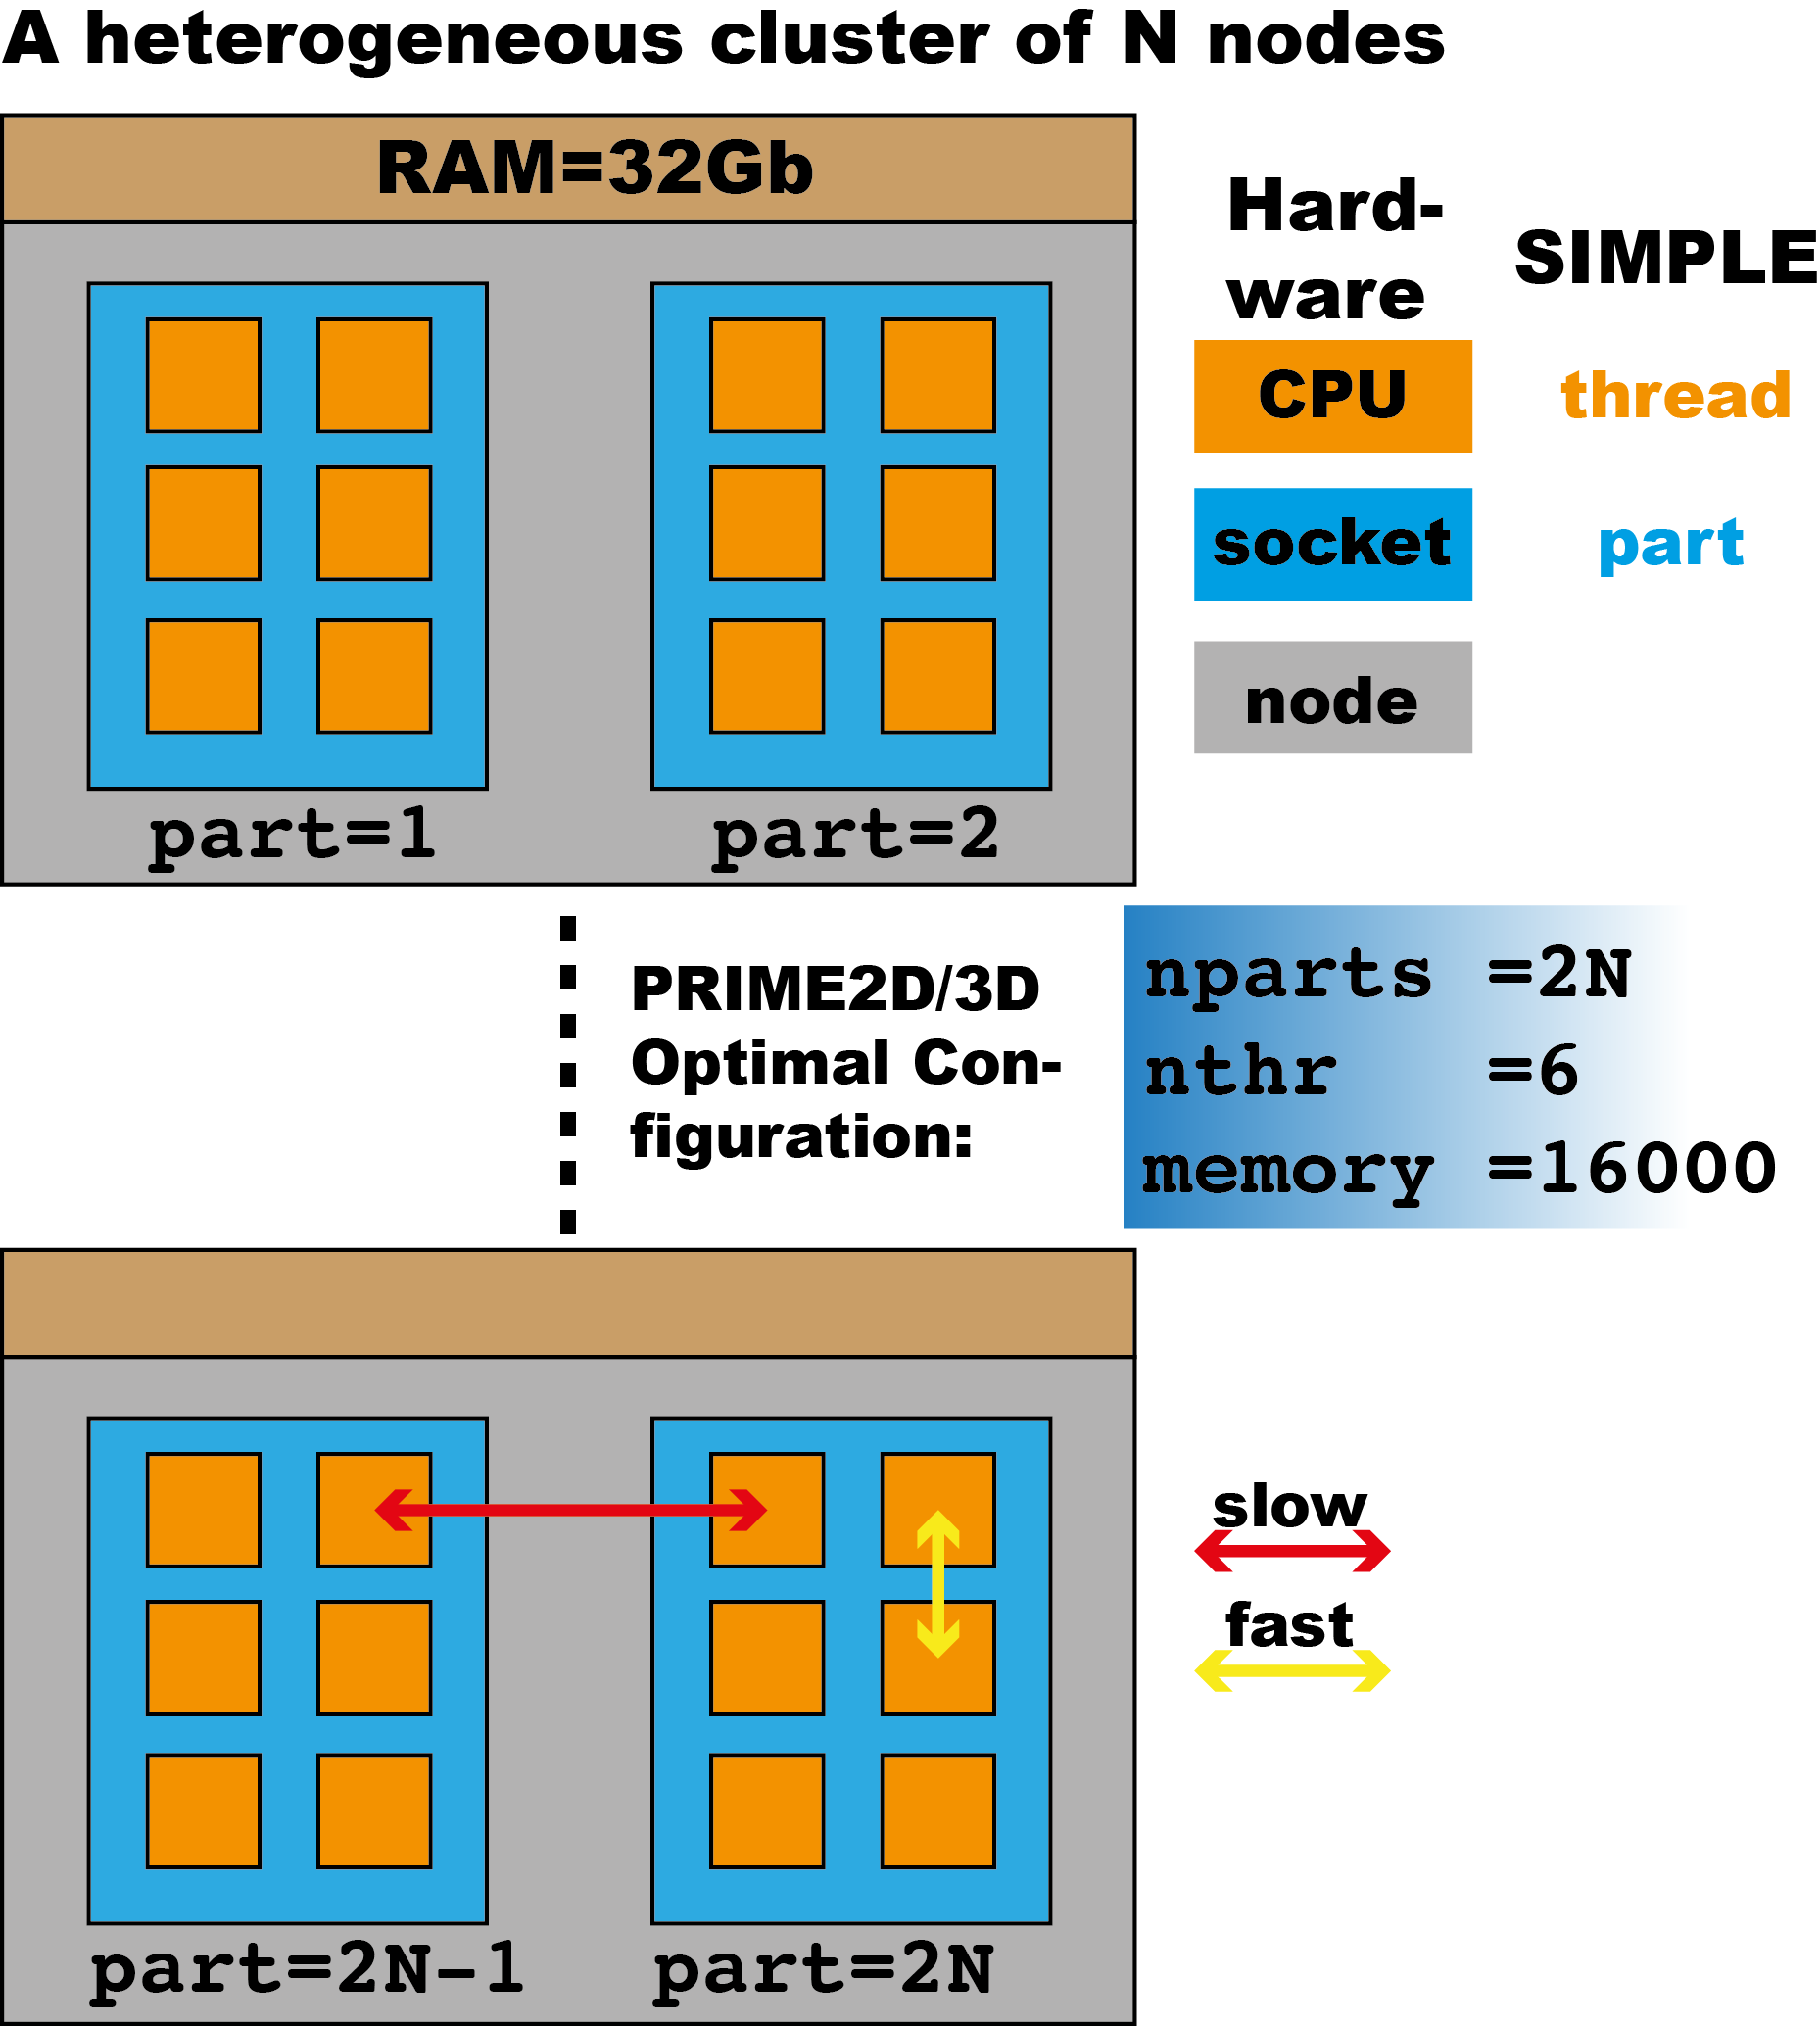
\includegraphics[keepaspectratio=true,scale=0.6]{./CPUtopo/cputopo}
\caption{\textbf{Configuration of the parallel PRIME-2D/3D execution on a heterogeneous cluster.} We here represent the nodes in  a heterogeneous cluster by two sockets with six CPUs each and 32Gb RAM/node. The best performance of PRIME--2D/3D is going to be obtained by partitioning  the jobs into \texttt{npart=2N} partitions, where \texttt{N} is the number of nodes. Each partition will then execute six threads \texttt{nthr=6} and these six threads will get access to half the RAM on the node (\texttt{memory=16000}) because we have two sockets per node that need to share the RAM between them}
\end{SCfigure}
If you are unsure how to configure your SIMPLE execution please file a help ticket.

\section{DDD Movie Pre-processing}

\subsection{Motion Correction}
During image acquisition, beam induced motion, charging and stage drift introduce blurring in the integrated movies. The individual frames need to be aligned with respect to one another in order to restore high-resolution information. Because of radiation damage, the electron dose is kept low during image acquisition, resulting in a very low signal-to-noise ratio (SNR) of the individual movie frames. SIMPLE implements a program called \prgname{unblur} for simultaneous motion-correction, frame-weighting and dose-weighting, with the objective of maximising the SNR of the integrated movie in a motion- and dose-dependent manner. Input is a text file \texttt{filetab}, simply listing the individual movies in \texttt{*.mrc} format, the pixel-to-pixel (or sampling) distance \texttt{smpd} (in \AA{}), the number of CPU threads to use \texttt{nthr}, the template name of the outputted files \texttt{fbody}, in addition to a number of other optional parameters that we will not be concerned with here. If we execute \texttt{simple\_distr\_exec prg=unblur} in the prompt, we obtain brief instructions for how to run the program:
\begin{verbatim}
bash-3.2$ simple_distr_exec prg=unblur_movies
USAGE:
bash-3.2$ simple_distr_exec prg=simple_program key1=val1 key2=val2 ...

REQUIRED
filetab = list of files(*.txt/*.asc)
smpd    = sampling distance, same as EMANs apix(in A)
nparts  = # partitions in distributed exection

OPTIONAL
nthr       = # OpenMP threads{1}
ncunits    = # computing units, can be < nparts{nparts}
fbody      = file body
dose_rate  = dose rate(in e/A2/s)
exp_time   = expusure time(in s)
lpstart    = start low-pass limit(in A){15}
lpstop     = stop low-pass limit(in A){8}
trs        = maximum halfwidth shift(in pixels)
kv         = acceleration voltage(in kV){300.}
pspecsz    = size of power spectrum(in pixels)
numlen     = length of number string
startit    = start iterating from here
scale      = image scale factor{1}
nframesgrp = # frames to group before unblur(Falcon 3){0}
fromf      = start frame index
tof        = stop frame index
nsig       = # sigmas
\end{verbatim}
Output consists of four files per movie (\texttt{movie1.mrc} in this example):
\begin{enumerate}
\item \texttt{<fbody>\_intg1.mrc} is the frame-weighted, motion-corrected sum
\item \texttt{<fbody>\_forctf1.mrc} is the un-weighted sum of the aligned individual frames
\item \texttt{<fbody>\_pspec1.mrc} is the power-spectrum of the uncorrected unweighted movie sum (left) and the corrected weighted movie sum (right)
\item \texttt{<fbody>\_thumb1.mrc} is a down-scaled version of  \texttt{<fbody>\_intg1.mrc}
\end{enumerate}
The \texttt{*forctf*} output is created because weighting the frames may degrade the contrast transfer function (CTF) signal and this file will therefore later be used to determine the CTF parameters of the integrated movie. The \texttt{*intg*} image is the dose-weighted one you will use for particle picking and extract your identified individual particle images from. The \texttt{*pspec*} and \texttt{*thumb*} outputs are diagnostic. Please, check so that the Thon rings are concentric and have similar radial intensity distribution in any given resolution shell after alignment (right part of power-spectrum)\textemdash{}if not, trash the image. If you have downloaded the example data folder, please execute

\begin{verbatim}
bash-3.2$ cd 1_DDD-movie-proc/
bash-3.2$ ls
data
bash-3.2$ ls ./data/
4comparison  boxfiles  info.txt  movie1.mrc  movie2.mrc
bash-3.2$ cat ./data/info.txt 
molecule: proteasome
exp_time=7.6s
dose_rate=7e/A2/s
kv=300
cs=2.7
smpd=5.26
fraca=0.1
bash-3.2$ ls ./data/movie* > movies.txt
bash-3.2$ cat movies.txt 
./data/movie1.mrc
./data/movie2.mrc
\end{verbatim}

These movies are of proteasome molecules in ice (EMPIAR-10025), exposed for \texttt{exp\_time=7.6} s with a dose rate of \texttt{dose\_rate=7} e/\AA{}$^2$/s. The  electron microscope used to acquire these images has an acceleration voltage of \texttt{kv=300} kV and a spherical aberration constant of \texttt{cs=2.7} mm. We have downscaled these images for more rapid processing to a sampling distance of \texttt{smpd=5.26} \AA{} and we will assume 10\% amplitude contrast when fitting the CTF \texttt{fraca=0.1}. First, we need to create a file table, listing the movies to be processed with  \prgname{unblur}.
\begin{verbatim}
bash-3.2$ ls data/movie* > movies.txt
\end{verbatim}
To see what this file contains, execute:
\begin{verbatim}
bash-3.2$ cat movies.txt 
data/movie1.mrc
data/movie2.mrc
\end{verbatim}
Next, we execute the program.
\begin{verbatim}
bash-3.2$ simple_distr_exec prg=unblur filetab=movies.txt smpd=5.26 
nparts=2 nthr=12 fbody=proteasome dose_rate=7 exp_time=7.6 kv=300 
fbody=proteasome
\end{verbatim}
The first thing that happens is that all individual movie frames are read in and Fourier transformed. The algorithm is iterative and based on registration of the individual frames to a weighted average, where the weights are determined based on the agreement between the frames and the average. The algorithm automatically updates the resolution limit as the alignment accuracy improves, \textit{i.e.} using only low-resolution Fourier components at first when the alignment errors are large and large movements need to be identified. It then successively updates the resolution limit as the alignment accuracy improves. When no improvements can be identified, the procedure stops. The outputted image files are:
\begin{verbatim}
bash-3.2$ ls
data                    proteasome_forctf2.mrc  proteasome_pspec2.mrc    
movies.txt              proteasome_intg1.mrc    proteasome_thumb1.mrc
simple_unidoc.txt       proteasome_intg2.mrc    proteasome_thumb2.mrc
proteasome_forctf1.mrc  proteasome_pspec1.mrc   simple_distr_config.env
\end{verbatim}
The first images we inspect are the power spectra. For visualisation, use the EMAN2 program \texttt{e2display.py}. Execute \texttt{e2display.py} in the current working directory, click on one of the \texttt{*pspec*} files and then \texttt{Show 2D}.
\begin{SCfigure}[][h]

\includegraphics[keepaspectratio=true,scale=0.3]{./pspec/pspec}
\caption{The left part of the power spectrum represents the movie integrated without applying the alignment parameters, whereas the right part is the aligned integrated movie. We see that the motion correction restores coherence, giving radially symmetric Thon rings extending to much higher resolution.}
\end{SCfigure}
To get an idea of the effect of the movie pre-processing in real-space, expand the data folder from within \texttt{e2display.py}, then expand the \texttt{4comparison} folder and click on the \texttt{proteasome\_straight\_intg1.mrc} file, followed by \texttt{Show 2D+}. Do the same for the corrected movie \texttt{proteasome\_intg1.mrc} and compare the two images.
\newpage{}
\begin{figure}
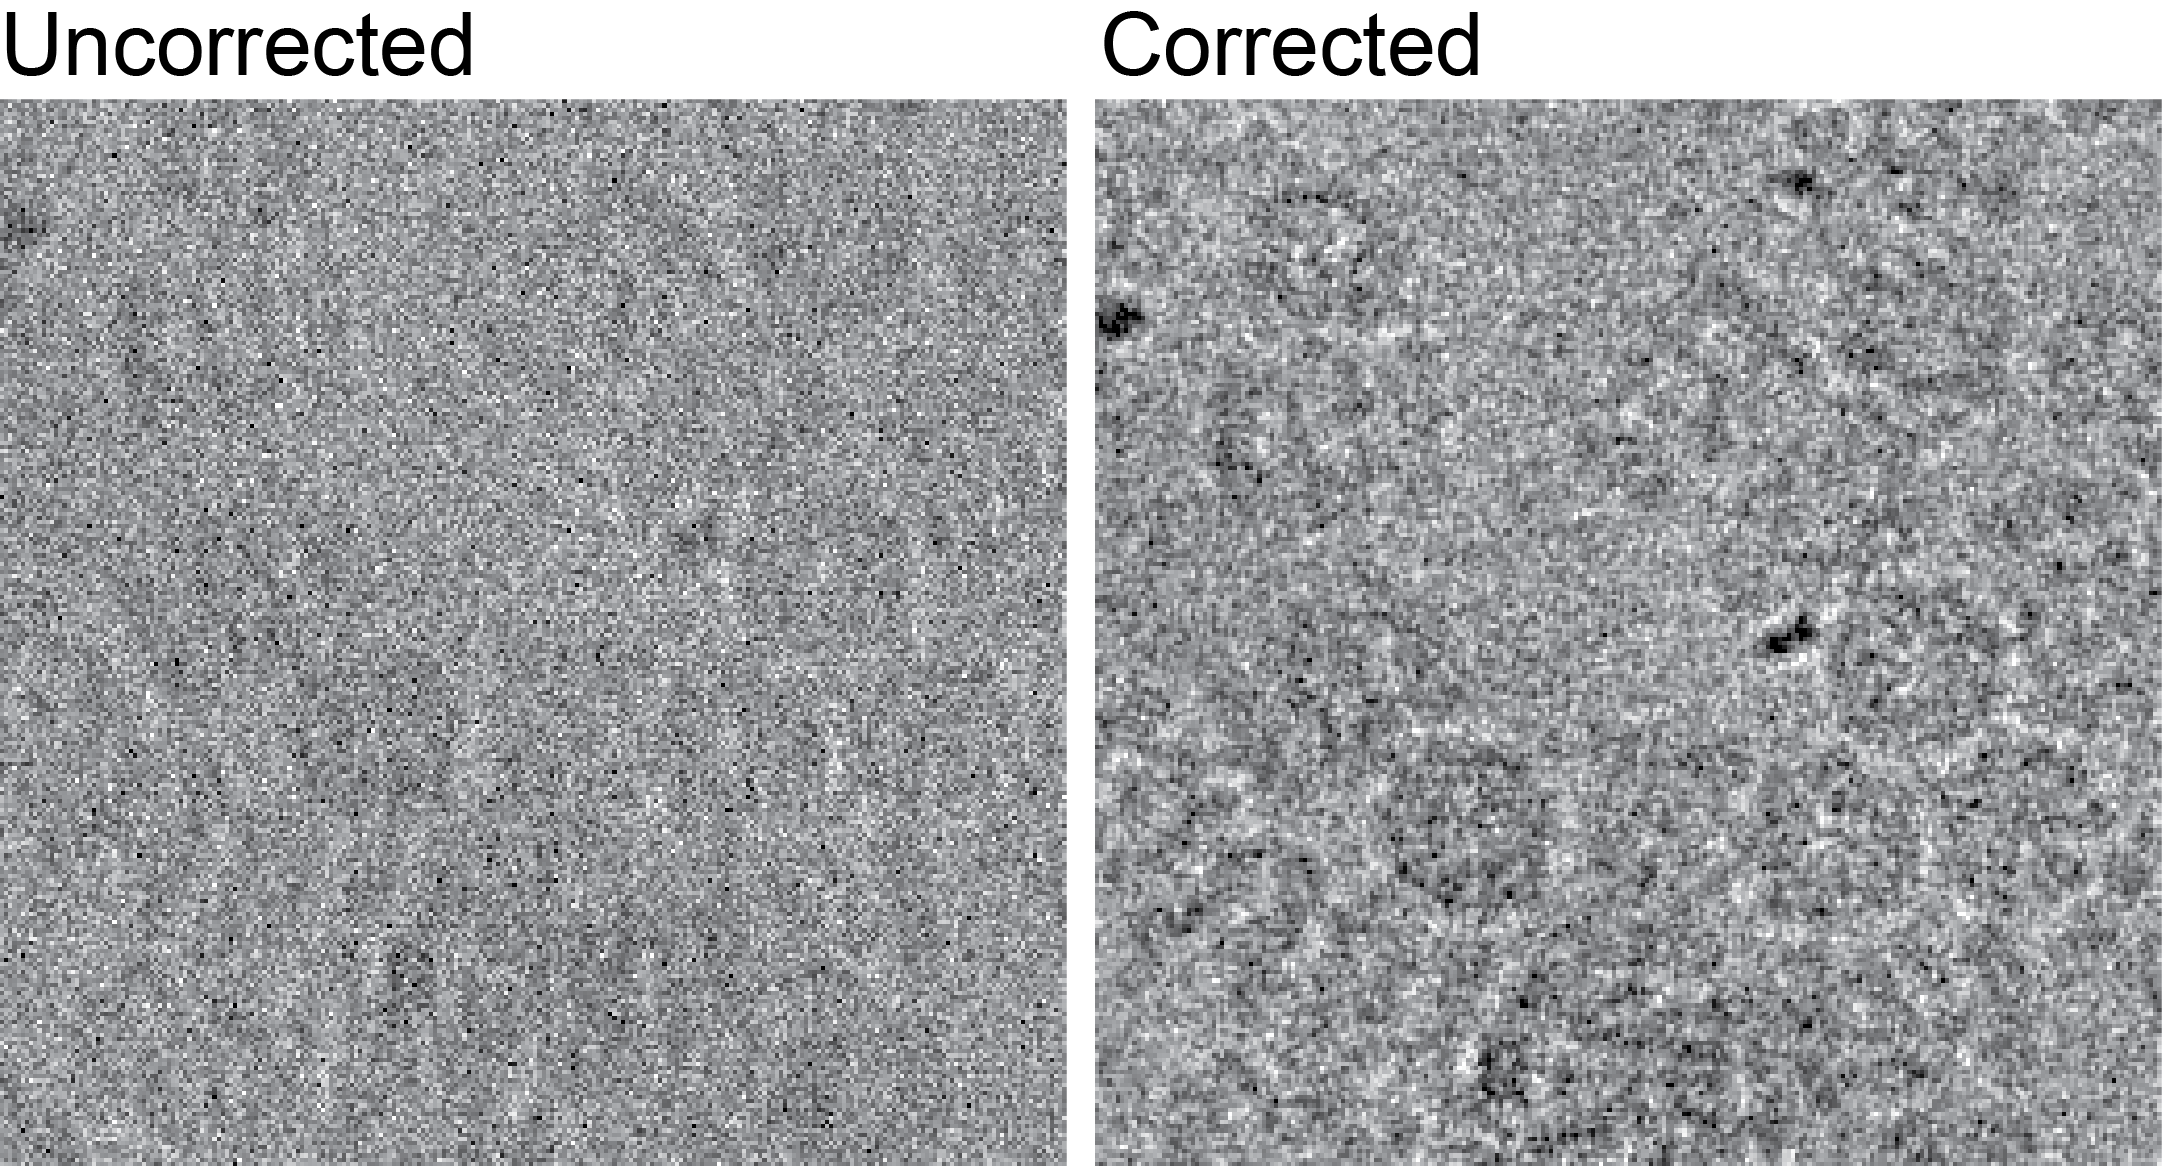
\includegraphics[keepaspectratio=true,scale=0.7]{./straightvsintg/straightvsintg}
\caption{The uncorrected movie, integrated without alignment, is blurred and lacks high-resolution contrast, whereas the corrected movie has much higher contrast and better definition.}
\end{figure}

\begin{tcolorbox}[breakable,colback=white,colframe=orange,width=\dimexpr\textwidth+12mm\relax,enlarge left by=-6mm]
\subsection{Using SIMPLE in the Wild\textemdash{}Power Spectrum Analysis and Movie Selection}
In a real-life scenario, all images in a data set are never perfect. A truck may come driving by the EM suite and cause drift, someone may pass the EM room transporting a big piece of metal, causing the energy filter to become misaligned, or the pump of the autoloader may have been accidentally turned on. The list could be made long. Therefore, it is important that we take a good look at our data. The first round of screening is usually done by looking at power spectra\textemdash{}the \texttt{*pspec*} files produced by \prgname{unblur}. Typically, you will have executed \texttt{unblur} in distributed mode in a cluster environment (described below) and a stack of power spectra called \texttt{unblur\_pspecs.mrc} has then been produced. We use EMAN2 to look at the power spectra and Steve will introduce you to EMAN2 in the next session but you can use whatever GUI you like to make the selection. SIMPLE supports MRC and SPIDER files but does not allow you to mix formats, so if you need to convert between MRC and SPIDER file formats, use SIMPLE program \prgname{convert}
\begin{verbatim}
bash-3.2$ simple_exec prg=convert
USAGE:
bash-3.2$ simple_exec prg=simple_program key1=val1 key2=val2 ...

OPTIONAL
stk    = particle stack with all images(ptcls.ext)
vol1   = input volume no1(invol1.ext)
outstk = output image stack
outvol = output volume{outvol.ext}
\end{verbatim}
Once you have made the selection and have the two stacks \texttt{unblur\_pspecs.mrc} and \texttt{good\_pspecs.mrc} or whatever you select to call them you can propagate the selection to your \texttt{*intg*} and \texttt{*forctf*} files using SIMPLE program \prgname{select}
\begin{verbatim}
bash-3.2$ simple_exec prg=select
USAGE:
bash-3.2$ simple_exec prg=simple_program key1=val1 key2=val2 ...

REQUIRED
stk  = particle stack with all images(ptcls.ext)
stk2 = 2nd stack(in map2ptcls/select: selected(cavgs).ext)

OPTIONAL
nthr       = nr of OpenMP threads{1}
stk3       = 3d stack (in map2ptcls/select: (cavgs)2selectfrom.ext)
filetab    = list of files(*.txt/*.asc)
outfile    = output document
outstk     = output image stack
dir_select = move selected files to here{selected}
dir_reject = move rejected files to here{rejected}
\end{verbatim}
You would then execute \prgname{select} twice. In the first pass to select your \texttt{*intg*} files:
\begin{verbatim}
bash-3.2$ ls *intg* > intg_movies.txt
bash-3.2$ simple_exec prg=select stk=unblur_pspecs.mrc stk2=good_pspecs.mrc nthr=8 
filetab=intg_movies.txt dir_select=intg_selected dir_reject=intg_rejected
\end{verbatim}
and in the second pass to select your \texttt{*forctf*} files:
\begin{verbatim}
bash-3.2$ ls *forctf* > forctf_movies.txt
bash-3.2$ simple_exec prg=select stk=unblur_pspecs.mrc stk2=good_pspecs.mrc nthr=8 
filetab=forctf_movies.txt dir_select=forctf_selected dir_reject=forctf_rejected
\end{verbatim}
\end{tcolorbox}

\begin{SCfigure}[][h]
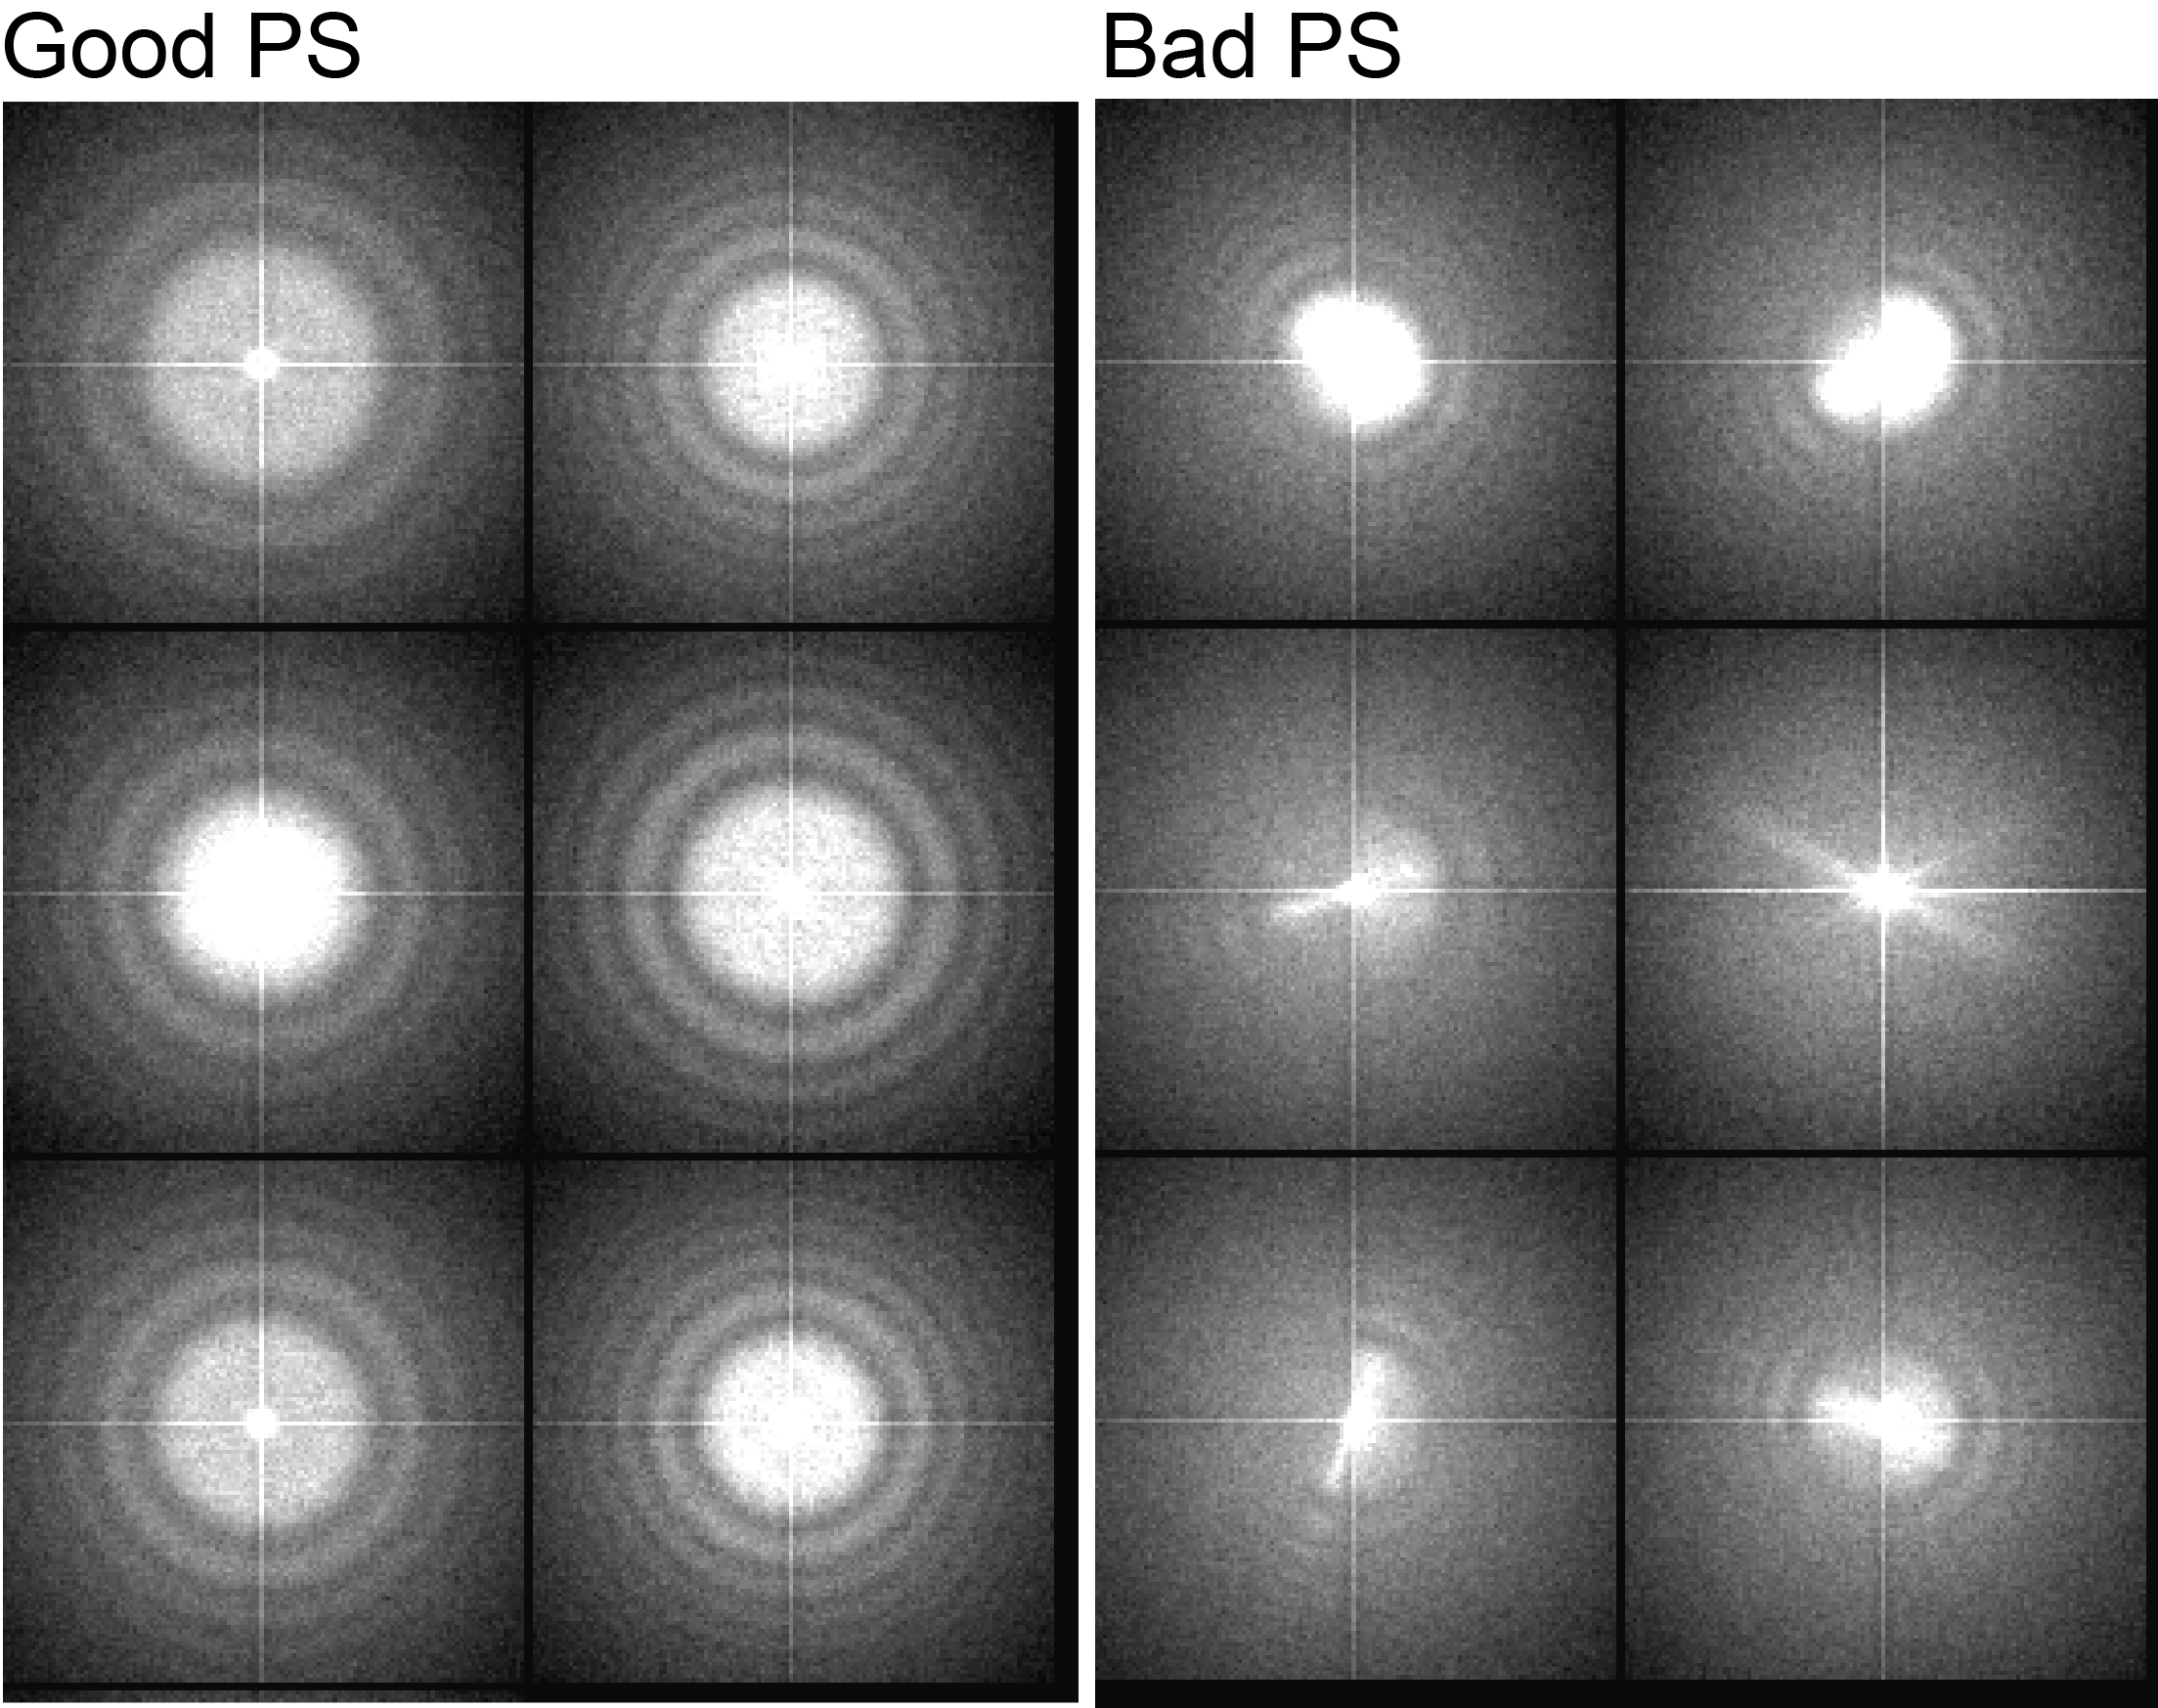
\includegraphics[keepaspectratio=true,scale=0.6]{./spectra/pspecs}
\caption{Examples of good power spectra (left) and bad power spectra (right)}
\end{SCfigure}

\subsection{CTF Parameter Determination}
The contrast transfer function (CTF) mathematically describes how aberrations in a transmission electron microscope modify the recorded image. The assumption we rely on is that the image is a projection of the Coulomb potential distribution of the specimen, convoluted (multiplied in Fourier space) with the CTF and with Gaussian noise added. All 3D reconstruction methodology rely on this or slight variations of this assumption. The CTF is an oscillatory function (we saw the effect of it in the power spectrum in Figure 1) and the frequency of the oscillations depends on the spherical aberration constant \texttt{cs} in mm, which is an instrument specific constant, and  the defocus in microns, which we systematically vary during image acquisition. The reason that we vary the defocus during data collection is that we want to avoid systematic lack of information in certain resolution regions, as no information other than noise is present in the zero crossings of the CTF. By varying the defocus we shift the positions of the zero crossings of the CTF. If astigmatism is present in the image, the Thon rings are no longer radially symmetric but elliptical and we need to take this into account as well.

The CTF has two components: one phase contrast component (giving rise to the same kind of contrast as in a medical X-ray image)  and one amplitude contrast component (giving rise to the same kind of contrast as when you put your hand on a projector, omitting photons to create a shadow image). Most of the contrast in biological cryo-EM are due to change in phase. In fact, the fraction of amplitude contrast has been measured to be around 10\% for proteins. In summary, we need six parameters to determine the parameters of the CTF: the acceleration voltage \texttt{kv}, the spherical aberration constant \texttt{cs}, the fraction of amplitude contrast \texttt{fraca}, the defocus in the x-direction \texttt{dfx}, the defocus in the y-direction \texttt{dfy} and the angle of astigmatism \texttt{angast}. The \texttt{kv}, \texttt{cs}, and \texttt{fraca} we treat as constants. Although we measure the defocus and astigmatism during data acquisition, the accuracies of these measurements are too crude to be useful for image processing. However, the protein itself, the carbon support and the ice scatters sufficiently for us to be able to generate a power spectrum that accurately represents the CTF power. This is typically done by extracting overlapping boxes from the micrograph, for every box calculating a power spectrum and averaging all power spectra over a micrograph to enhance the CTF signal. Using a parametric model for the CTF of the form
\bea
CTF=A_{phase}sin(\phi)+A_{amp}cos(\phi)
\eea
where $A_{phase}=0.9$, $A_{amp}=0.1$ and the phase shift $\phi$
\bea
\phi=\pi{}\lambda{}s^{2}(D-\frac{\lambda{}^{2}s^{2}C_{s}}{2})
\eea
where $\lambda{}$ is the electron wavelength, $s$ is spatial frequency, $D$ is defocus and $C_{s}$ is the spherical aberration constant, we can determine  the parameters we need.

\begin{figure}
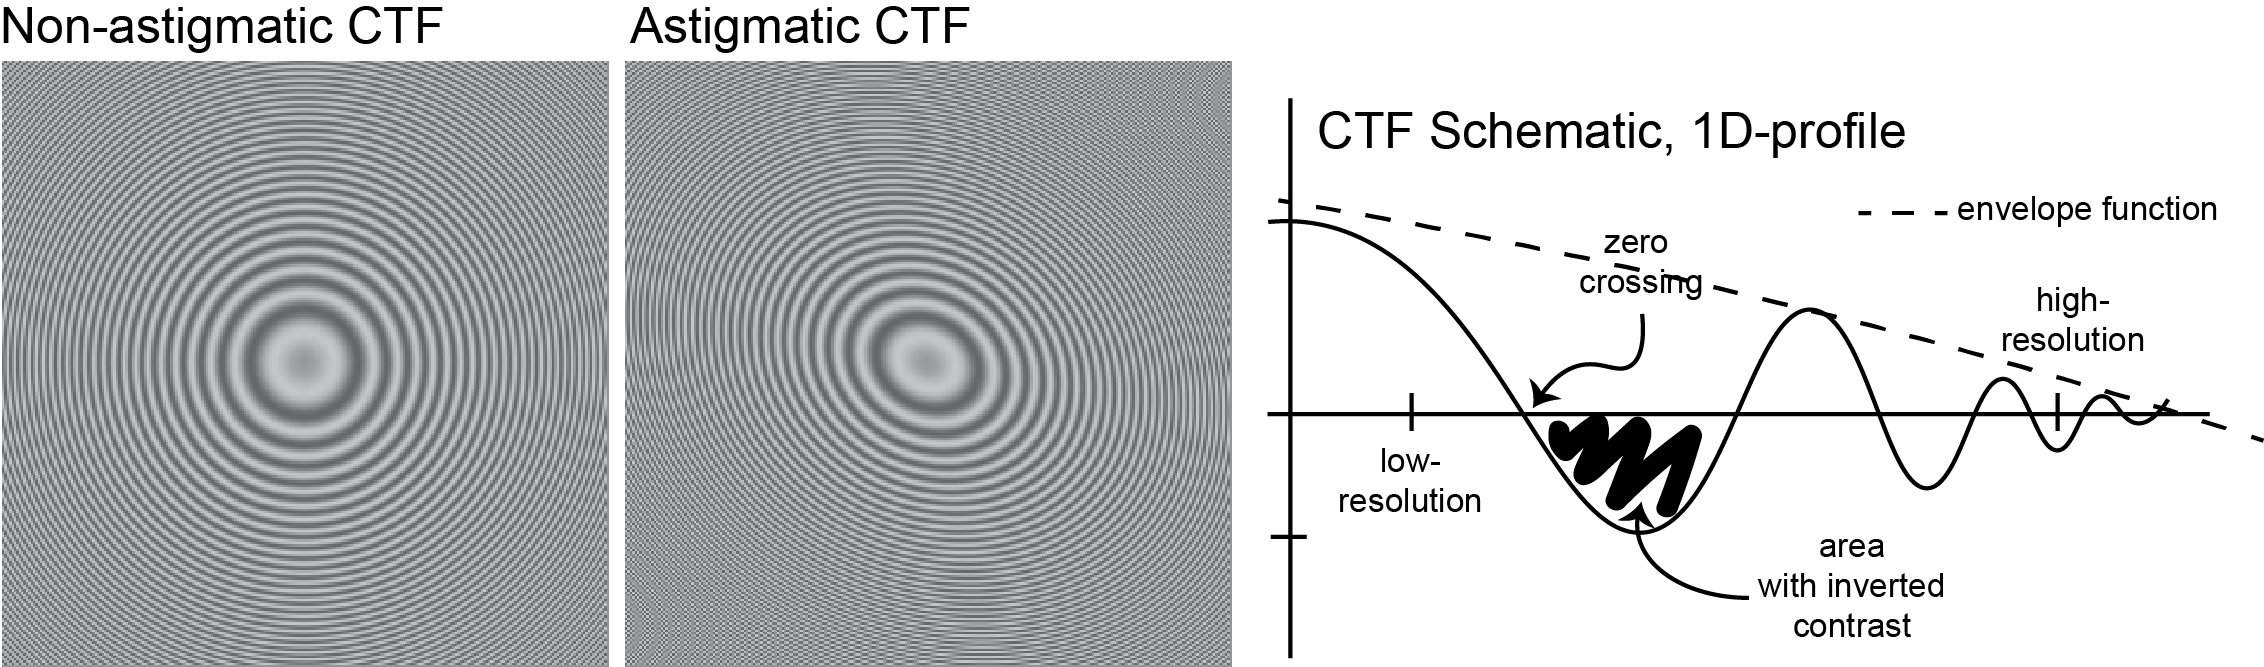
\includegraphics[keepaspectratio=true,scale=0.8 ]{./astigctf/astigctf}
\caption{Non-astigmatic CTF (left) vs. astigmatic CTF (middle) and schematic 1D CTF profile (right)}
\end{figure}

SIMPLE implements a wrapper program called \prgname{ctffind} that executes CTFFIND4 \citep{rohou2015ctffind4} version 4.1.X, producing a SIMPLE conforming CTF parameter document \texttt{deftab}. Input is a text file \texttt{filetab}, simply listing the individual integrated movies in \texttt{*.mrc} format, the pixel-to-pixel (or sampling) distance \texttt{smpd} (in \AA{}), the acceleration voltage of the electron microscope \texttt{kv} (in kV), the spherical aberration constant \texttt{cs} in mm and the fraction of amplitude contrast \texttt{fraca} in addition to a number of other optional parameters that we will not be concerned with here. If we execute \texttt{simple\_distr\_exec prg=ctffind} in the prompt, we obtain brief instructions for how to run the program:
\begin{verbatim}
bash-3.2$ simple_exec prg=ctffind
USAGE:
bash-3.2$ simple_distr_exec prg=simple_program key1=val1 key2=val2 ...

REQUIRED
filetab = list of files(*.txt/*.asc)
smpd    = sampling distance, same as EMANs apix(in A)
kv      = acceleration voltage(in kV){300.}
cs      = spherical aberration constant(in mm){2.7}
fraca   = fraction of amplitude contrast used for fitting CTF{0.07}
nparts  = # partitions in distributed exection

OPTIONAL
ncunits    = # computing units, can be < nparts{nparts}
pspecsz    = size of power spectrum(in pixels)
hp         = high-pass limit(in A)
lp         = low-pass limit(in A)
dfmin      = minimum expected defocus(in microns)
dfmax      = maximum expected defocus(in microns)
astigstep  = step size for astigamtism search(in microns)
expastig   = expected astigmatism(in microns)
phaseplate = images obtained with phaseplate(yes|no){no}
\end{verbatim}
Output is a text file with defocus parameters \texttt{ctffind\_output.txt}. First, we need to create a file table, listing the integrated movies to be processed with  \prgname{ctffind}.
\begin{verbatim}
bash-3.2$ ls proteasome_forctf* > ctf_movies.txt
\end{verbatim}
As explained above, the \texttt{*forctf*} output is created because weighted averaging may degrade the contrast transfer function (CTF) signal and this un-weighted average is therefore used to determine the CTF parameters of the integrated movie. Next, we execute the program.
\begin{verbatim}
bash-3.2$ simple_distr_exec prg=ctffind filetab=ctf_movies.txt smpd=5.26
kv=300 cs=2.7 fraca=0.1 nparts=2
\end{verbatim}
Output is the file \texttt{ctffind\_output.txt}.

In SIMPLE, we have yet to implement a particle picker but rely on EMAN1.9 and EMAN2 for particle identification. However, if you have \texttt{*.box} files obtained with EMAN you can extract the particle images and their associated CTF parameters using SIMPLE. To illustrate this functionality, we have prepared box files in the \texttt{data} folder for use in conjunction with SIMPLE program \prgname{extract}. As before, we need to prepare file tables. First, we prepare a file table for the motion corrected integrated movies:
\begin{verbatim}
bash-3.2$ ls proteasome_intg* > intg_movies.txt
\end{verbatim}
Second, for the box files:
\begin{verbatim}
bash-3.2$ ls ./data/boxfiles/*box > boxfiles.txt
\end{verbatim}
Finally, we execute the program:
\begin{verbatim}
bash-3.2$ simple_exec prg=extract filetab=intg_movies.txt boxtab=boxfiles.txt
smpd=5.26 ctffind_doc=ctffind_output.txt 
>>> DONE PROCESSING PARAMETERS
>>> DONE BUILDING GENERAL TOOLBOX
  100%  |==================================================| done.
       _______ _____ _______  _____         _______
       |______   |   |  |  | |_____] |      |______
       ______| __|__ |  |  | |       |_____ |______
 
 _)_ ( _   _     ) o  _             _   _   _   o  _   _
 (_   ) ) )_)   (  ( ) ) (_( \)    )_) ) ) (_(  ( ) ) )_)
         (_                  (\   (_         _)      (_

**** SIMPLE_EXTRACT NORMAL STOP ****
\end{verbatim}
Output is a particle stack \texttt{sumstack.mrc} and its associated parameter file \texttt{extract\_params.txt}.

\section{2D Analysis with PRIME2D}
Algorithms that can rapidly discover clusters corresponding to sets of images with similar projection direction and conformational state play an important role in single-particle analysis. Identification of such clusters allows for enhancement of the signal-to-noise ratio (SNR) by averaging and gives a first glimpse into the character of a dataset. Therefore, clustering algorithms play a pivotal role in initial data quality assessment, \textit{ab initio} 3D reconstruction and analysis of heterogeneous single-particle populations. SIMPLE implements a probabilistic algorithm for simultaneous 2D alignment and clustering, called \prgname{prime2D}. The version we are going to use here is an improved version of the published code \citep{reboul2016stochastic}. Grouping tens of thousands of images into several hundred clusters is a computationally intensive job. Therefore, we will now introduce the execution route for running SIMPLE jobs in a distributed computing environment.

\subsection{PRIME2D Analysis of TRPV1 Membrane Receptor Images}
The computers we are currently using have four i7 processors in a single socket, hyper-threaded so it looks like we have eight. We are now going to pretend that we have two CPU sockets with four CPUs each for the purpose of demonstration. Go to the \texttt{PRIME2D} directory and check things out.
\begin{verbatim}
bash-3.2$ cd ../2_PRIME2D/
bash-3.2$ ls
data/
bash-3.2$ ls data/
info.txt                 trpv1_extract_params.txt trpv1_ptcls.mrc
bash-3.2$ cat data/info.txt 
smpd=2.43
kv=300.
cs=2.0
fraca=0.1
ctf=flip
msk=36
box=128
\end{verbatim}
The key-value pair \texttt{ctf=flip} means that the images have been ``phase-flipped'', \textit{i.e.} the contrast bands inverted by the CTF have been reverted simply by multiplying the Fourier transform of the image with the sign of the CTF. The individual particle images are quite noisy and it is difficult to gain any understanding about the imaged structure from these images, which represent a subset of particles from a larger TRPV1 data set (EMPIAR-10005). 
\begin{SCfigure}[][h]
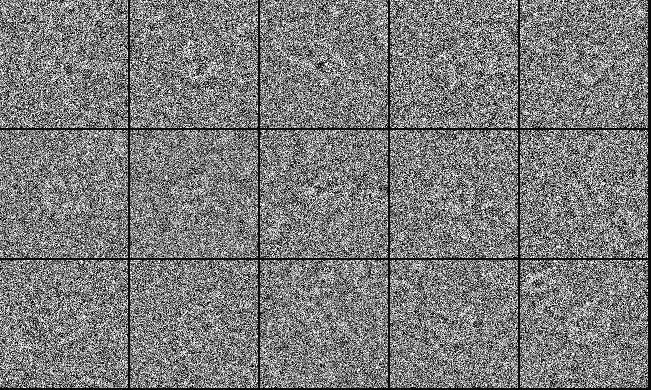
\includegraphics[keepaspectratio=true,scale=0.3]{./trpv1ptcls}
\caption{Individual TRPV1 particle images.}
\end{SCfigure}
In order to cluster the images, execute:
\begin{verbatim}
bash-3.2$ simple_distr_exec prg=prime2D stk=./data/trpv1_ptcls.mrc smpd=2.43 msk=36 
ncls=5 ctf=flip nparts=2 nthr=4 deftab=./data/trpv1_extract_params.txt
\end{verbatim}
For every iteration, we expect to see the following output in the terminal:
\begin{verbatim}
>>>
>>> ITERATION     10
>>>
DISTRIBUTED MODE :: submitting scripts:
distr_simple_script_1
distr_simple_script_2
appending output to nohup.out
appending output to nohup.out
>>> DONE PROCESSING PARAMETERS
**** SIMPLE_MERGE_ALGNDOCS NORMAL STOP ****
>>> DONE PROCESSING PARAMETERS
>>> DONE BUILDING GENERAL TOOLBOX
>>> DONE BUILDING HADAMARD PRIME2D TOOLBOX
**** SIMPLE_CAVGASSEMBLE NORMAL STOP ****
>>> DONE PROCESSING PARAMETERS
>>> DONE BUILDING GENERAL TOOLBOX
>>> JOINT    DISTRIBUTION OVERLAP:       0.6757
>>> CLASS    DISTRIBUTION OVERLAP:       0.8030
>>> IN-PLANE DISTRIBUTION OVERLAP:       0.5485
>>> AVERAGE IN-PLANE ANGULAR DISTANCE:     13.8
>>> PERCENTAGE OF SEARCH SPACE SCANNED:    89.6
>>> CORRELATION:                         0.5618
>>> CONVERGED: .NO.
**** SIMPLE_CHECK2D_CONV NORMAL STOP ****
\end{verbatim}
The distribution overlap represents the agreement between the alignment and clustering parameters from the present and previous iteration. The most important metric, however, is the fraction of search space scanned. \prgname{prime2D} is based on stochastic hill climbing optimisation, which relies on the so-called first improvement heuristic. This means that not all references are matched for each particle in each round but only as many as is required to find an improving solution, which is instantly accepted. Therefore, in the beginning of the search only few references need to be evaluated to find improving configurations (percentage of search space is low) whereas when convergence to a local (or global) optimum has been achieved most if not all references need to be evaluated (percentage of search space is high). Convergence is based on the class overlap and the fraction of search space scanned. Upon completion of the calculation, we see
\begin{verbatim}
>>> CONVERGED: .YES.
**** SIMPLE_CHECK2D_CONV NORMAL STOP ****
>>> DONE PROCESSING PARAMETERS
>>> DONE BUILDING GENERAL TOOLBOX
CLASS:     4 POP:  489
CLASS:     2 POP:  433
CLASS:     3 POP:  301
CLASS:     5 POP:  202
CLASS:     1 POP:  194
**** SIMPLE_RANK_CAVGS NORMAL STOP ****
       _______ _____ _______  _____         _______
       |______   |   |  |  | |_____] |      |______
       ______| __|__ |  |  | |       |_____ |______
 
 _)_ ( _   _     ) o  _             _   _   _   o  _   _
 (_   ) ) )_)   (  ( ) ) (_( \)    )_) ) ) (_(  ( ) ) )_)
         (_                  (\   (_         _)      (_

**** SIMPLE_DISTR_PRIME2D NORMAL STOP ****
\end{verbatim}
\begin{SCfigure}[][h]
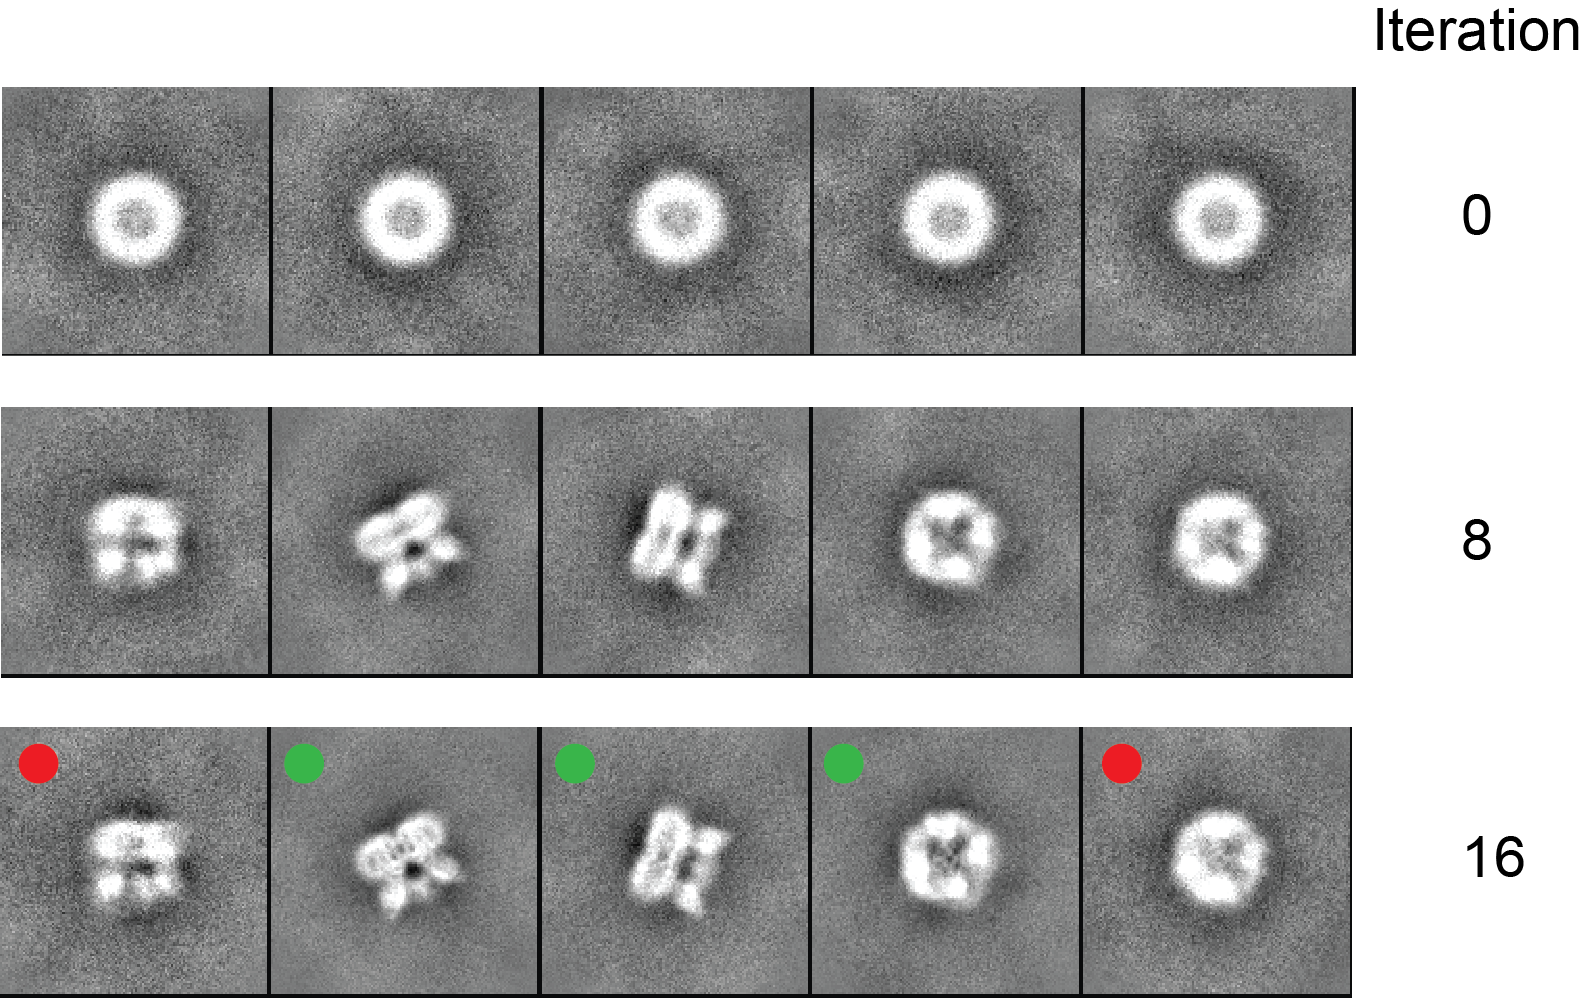
\includegraphics[keepaspectratio=true,scale=0.8]{./trpv1iters/trpv1iters}
\caption{TRPV1 class averages from the 0th (random initialisation), 8th, and and 16th (final) iteration of simultaneous 2D alignment and clustering with \prgname{prime2D}. Good class averages with clearly discernible projected secondary structure are marked with a green dot and class averages of lower quality are marked with a red dot.}
\end{SCfigure}

\begin{tcolorbox}[breakable,colback=white,colframe=orange,width=\dimexpr\textwidth+12mm\relax,enlarge left by=-6mm]
\subsection{Using SIMPLE in the Wild\textemdash{}Selecting Good Class Averages and Mapping the Selection to the Particles}
Most data sets contain images other than perfect particle images (false positives). Sometimes the particles tend to form micro-aggregations and are lying too close to each other or on top of each other. When automatic or semi-automatic particle identification procedures are used, ice-contaminations and carbon edges are often mistaken for particles. Therefore, it is good practice to first cluster the images into 100-200 classes and clean out the unwanted images before proceeding with grouping the data into a larger number of classes and calculating an initial 3D model. You can map the selection done on class averages back to the particle images using the SIMPLE program \prgname{map2ptcls}.
\begin{verbatim}
bash-3.2$ simple_exec prg=map2ptcls
USAGE:
bash-3.2$ simple_exec prg=simple_program key1=val1 key2=val2 ...

REQUIRED
stk    = particle stack with all images(ptcls.ext)
stk2   = 2nd stack(in map2ptcls/select: selected(cavgs).ext)
stk3   = 3d stack (in map2ptcls/select: (cavgs)2selectfrom.ext)
oritab = table (text file) of orientations(*.asc/*.txt)

OPTIONAL
oritab2   = 2nd table (text file) of orientations(*.asc/*.txt)
comlindoc = shc_clustering_nclsX.txt
doclist   = list of oritabs for different states
deftab    = text file with CTF info(*.txt/*.asc)
outfile   = output document
mul       = origin shift multiplication factor{1}
nthr      = nr of OpenMP threads{1}
\end{verbatim}
If your converged class averages from \prgname{prime2D} are \texttt{cavgs\_iter021.mrc} and your selected ones are \texttt{selected.mrc}, then you map the selection back to the particle images with the command:
\begin{verbatim}
bash-3.2$ simple_exec prg=map2ptcls stk=sumstack.mrc stk2=selected.mrc
stk3=cavgs_iter21.mrc oritab=prime2Ddoc_021.txt nthr=8
\end{verbatim}
creating a file \texttt{mapped\_ptcls\_params.txt} that you can input with flag \texttt{oritab} to \texttt{simple\_distr\_exec prg=prime2D} to execute a second pass of clustering using the clean set of particles.
\end{tcolorbox}

\section{\textit{Ab initio} 3D Reconstruction from Class Averages Using PRIME3D}
A major obstacle to achieving near-atomic resolution with single-particle cryo-EM is the problem of generating an accurate \textit{de novo} 3D reconstruction. Many cryo-EM structures are therefore solved by alignment of the images to \textit{a priori} models. The use of prior information, in the form of either a starting model from an independent source or an assumption of a particular point-group symmetry, is associated with the risk of introducing model bias. The model bias phenomenon is often illustrated by alignment of pure noise images to an image of Einstein. The image of Einstein is almost perfectly reproduced when the aligned noise images are averaged. It is often stated that low-pass filtering of X-ray maps, before they are used as starting models, eliminates model bias. This is a misunderstanding, as any model can be convincingly reproduced from noisy images \citep{henderson2013avoiding}. Most refinement software, such as FREALIGN \citep{Grigorieff:2007aa}, RELION \citep{Scheres:2012aa}, or projection matching \citep{penczek1994ribosome, Hohn:2007aa, Tang:2007aa}, depends on an accurate starting model for convergence to a high-resolution map. If the starting model is not supported by the images, there is a potent risk of introducing model bias. To what degree a starting model can bias the final 3D structure needs to be better characterised by methodological studies. We introduced the PRIME3D algorithm \citep{Elmlund:2013aa} to remove the requirement for \textit{a priori} structural knowledge and open the method to  the study of particles with novel structure. Robust algorithms for \textit{ab initio} 3D reconstruction are particularly important for the analysis of small particles with low symmetry.

\subsection{Analysis of Ribosome Class Averages Using the \prgname{ini3D\_from\_cavgs} Program}
SIMPLE was designed primarily for processing single-particle images of molecules with low or no internal symmetry. There are not an awful lot of data sets of asymmetric molecules publicly available, but one of the most popular specimens\textemdash{}one that we all recognise the structure of\textemdash{}is the ribosome. Although the initial idea with PRIME3D was to overcome the need for 2D clustering and generate an accurate 3D map straight from the noisy individual images, we have found that 2D analysis is extremely useful for weeding out bad data and enhancing SNR prior to 3D analysis. Processing class averages also makes 3D model validation easier as we can simply compare re-projections of the 3D map with the signal-enhanced class averages used to obtain the 3D reconstruction. We pre-calculated 2D class averages with PRIME 2D from a publicly available ribosome data set (EMPIAR-10028). These are located in the \texttt{3\_PRIME3D/data} folder. Please \texttt{cd} to this folder and have a look at the class averages with EMAN2.
\begin{figure}
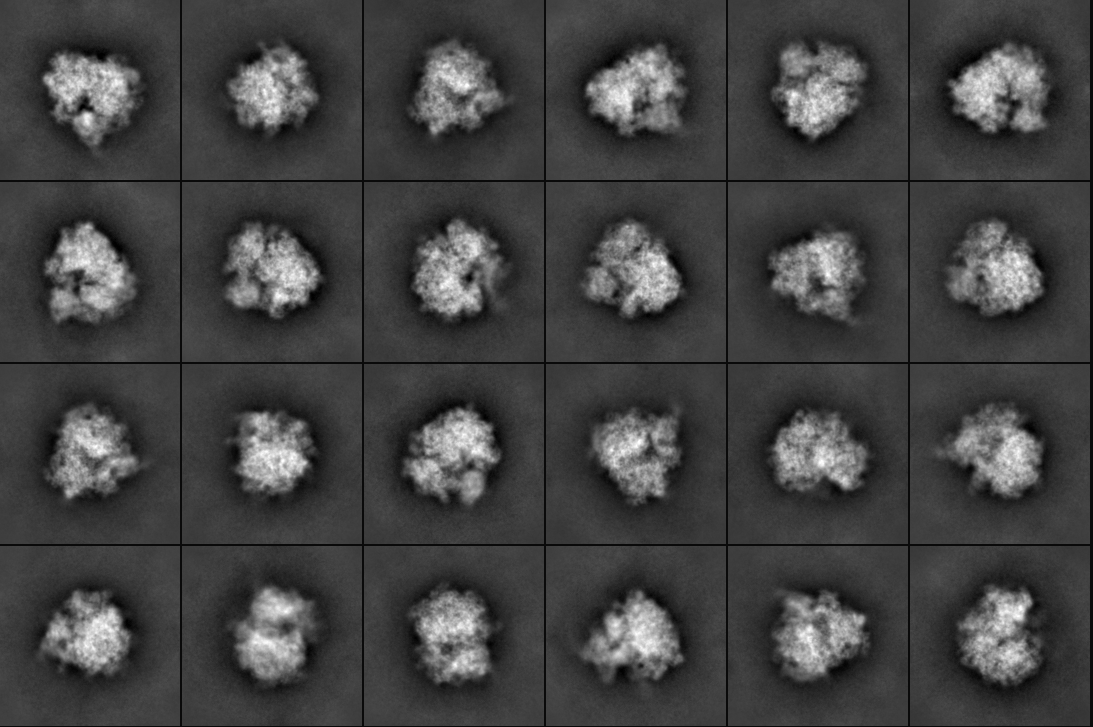
\includegraphics[keepaspectratio=true,scale=0.4]{./ribocavgs}
\caption{Ribosome class averages obtained with PRIME2D.}
\end{figure}
As before, the parameters associated with the class averages are listed in the \texttt{info.txt} file.
\begin{verbatim}
bash-3.2$ cat ./data/info.txt 
smpd=2.68
msk=80
pgrp=c1
\end{verbatim}
Input to \prgname{ini3D\_from\_cavgs} is a stack of class averages \texttt{stk}, sampling distance \texttt{smpd} in \AA{}, mask radius \texttt{msk} in pixels, point-group symmetry \texttt{pgrp} (\texttt{c1} in this case), the number of CPU threads \texttt{nthr} and the number of partitions to divide the job into \texttt{nparts}. The output from \prgname{ini3D\_from\_cavgs} is a 3D model \texttt{rec\_final.mrc} and re-projections of this model in the orientations assigned to the class averages \texttt{reprojs.mrc}. If we execute \texttt{simple\_distr\_exec prg=ini3D\_from\_cavgs} in the prompt, we obtain brief instructions for how to run the program:
\begin{verbatim}
bash-3.2$ simple_distr_exec prg=ini3D_from_cavgs
USAGE:
bash-3.2$ simple_distr_exec prg=simple_program key1=val1 key2=val2 ...

REQUIRED
stk    = particle stack with all images(ptcls.ext)
smpd   = sampling distance, same as EMANs apix(in A)
msk    = mask radius(in pixels)
pgrp   = point-group symmetry(cn|dn|t|o|i)
nparts = # partitions in distributed exection

OPTIONAL
nthr       = # OpenMP threads{1}
ncunits    = # computing units, can be < nparts{nparts}
hp         = high-pass limit(in A)
lp         = low-pass limit(in A)
lpstop     = stop low-pass limit(in A){8}
inner      = inner mask radius(in pixels)
width      = falloff of inner mask(in pixels){10}
nspace     = # projection directions
autoscale  = automatic down-scaling(yes|no){yes}
pgrp_known = point-group known a priori(yes|no){no}\end{verbatim}
In order to reconstruct an \textit{ab initio} 3D reconstruction, please execute:
\begin{verbatim}
bash-3.2$ simple_distr_exec prg=ini3D_from_cavgs stk=./data/pfrib80S_cavgs.mrc
smpd=2.68 msk=80 pgrp=c1 nthr=4 nparts=2 nthr_master=8
\end{verbatim}
For every iteration, we expect to see an output similar to that of PRIME2D in the terminal:
\begin{verbatim}
>>>
>>> ITERATION      4
>>>
DISTRIBUTED MODE :: submitting scripts:
distr_simple_script_1
distr_simple_script_2
appending output to nohup.out
appending output to nohup.out
>>> DONE PROCESSING PARAMETERS
**** SIMPLE_MERGE_ALGNDOCS NORMAL STOP ****
>>> DONE PROCESSING PARAMETERS
>>> DONE BUILDING GENERAL TOOLBOX
>>> DONE BUILDING RECONSTRUCTION TOOLBOX
**** SIMPLE_VOLASSEMBLE NORMAL STOP ****
>>> DONE PROCESSING PARAMETERS
>>> DONE BUILDING GENERAL TOOLBOX
>>> ANGLE OF FEASIBLE REGION:              14.6
>>> JOINT    DISTRIBUTION OVERLAP:       0.0775
>>> CLASS    DISTRIBUTION OVERLAP:       0.0600
>>> IN-PLANE DISTRIBUTION OVERLAP:       0.0950
>>> AVERAGE ANGULAR DISTANCE BTW ORIS:     63.7
>>> AVERAGE IN-PLANE ANGULAR DISTANCE:     16.8
>>> PERCENTAGE OF SEARCH SPACE SCANNED:    53.9
>>> CORRELATION:                         0.9536
>>> ANGULAR SDEV OF MODEL:                28.06
>>> UPDATE LOW-PASS LIMIT: .NO.
>>> CONVERGED: .NO.
**** SIMPLE_CHECK3D_CONV NORMAL STOP ****
\end{verbatim}
\begin{figure}[H]
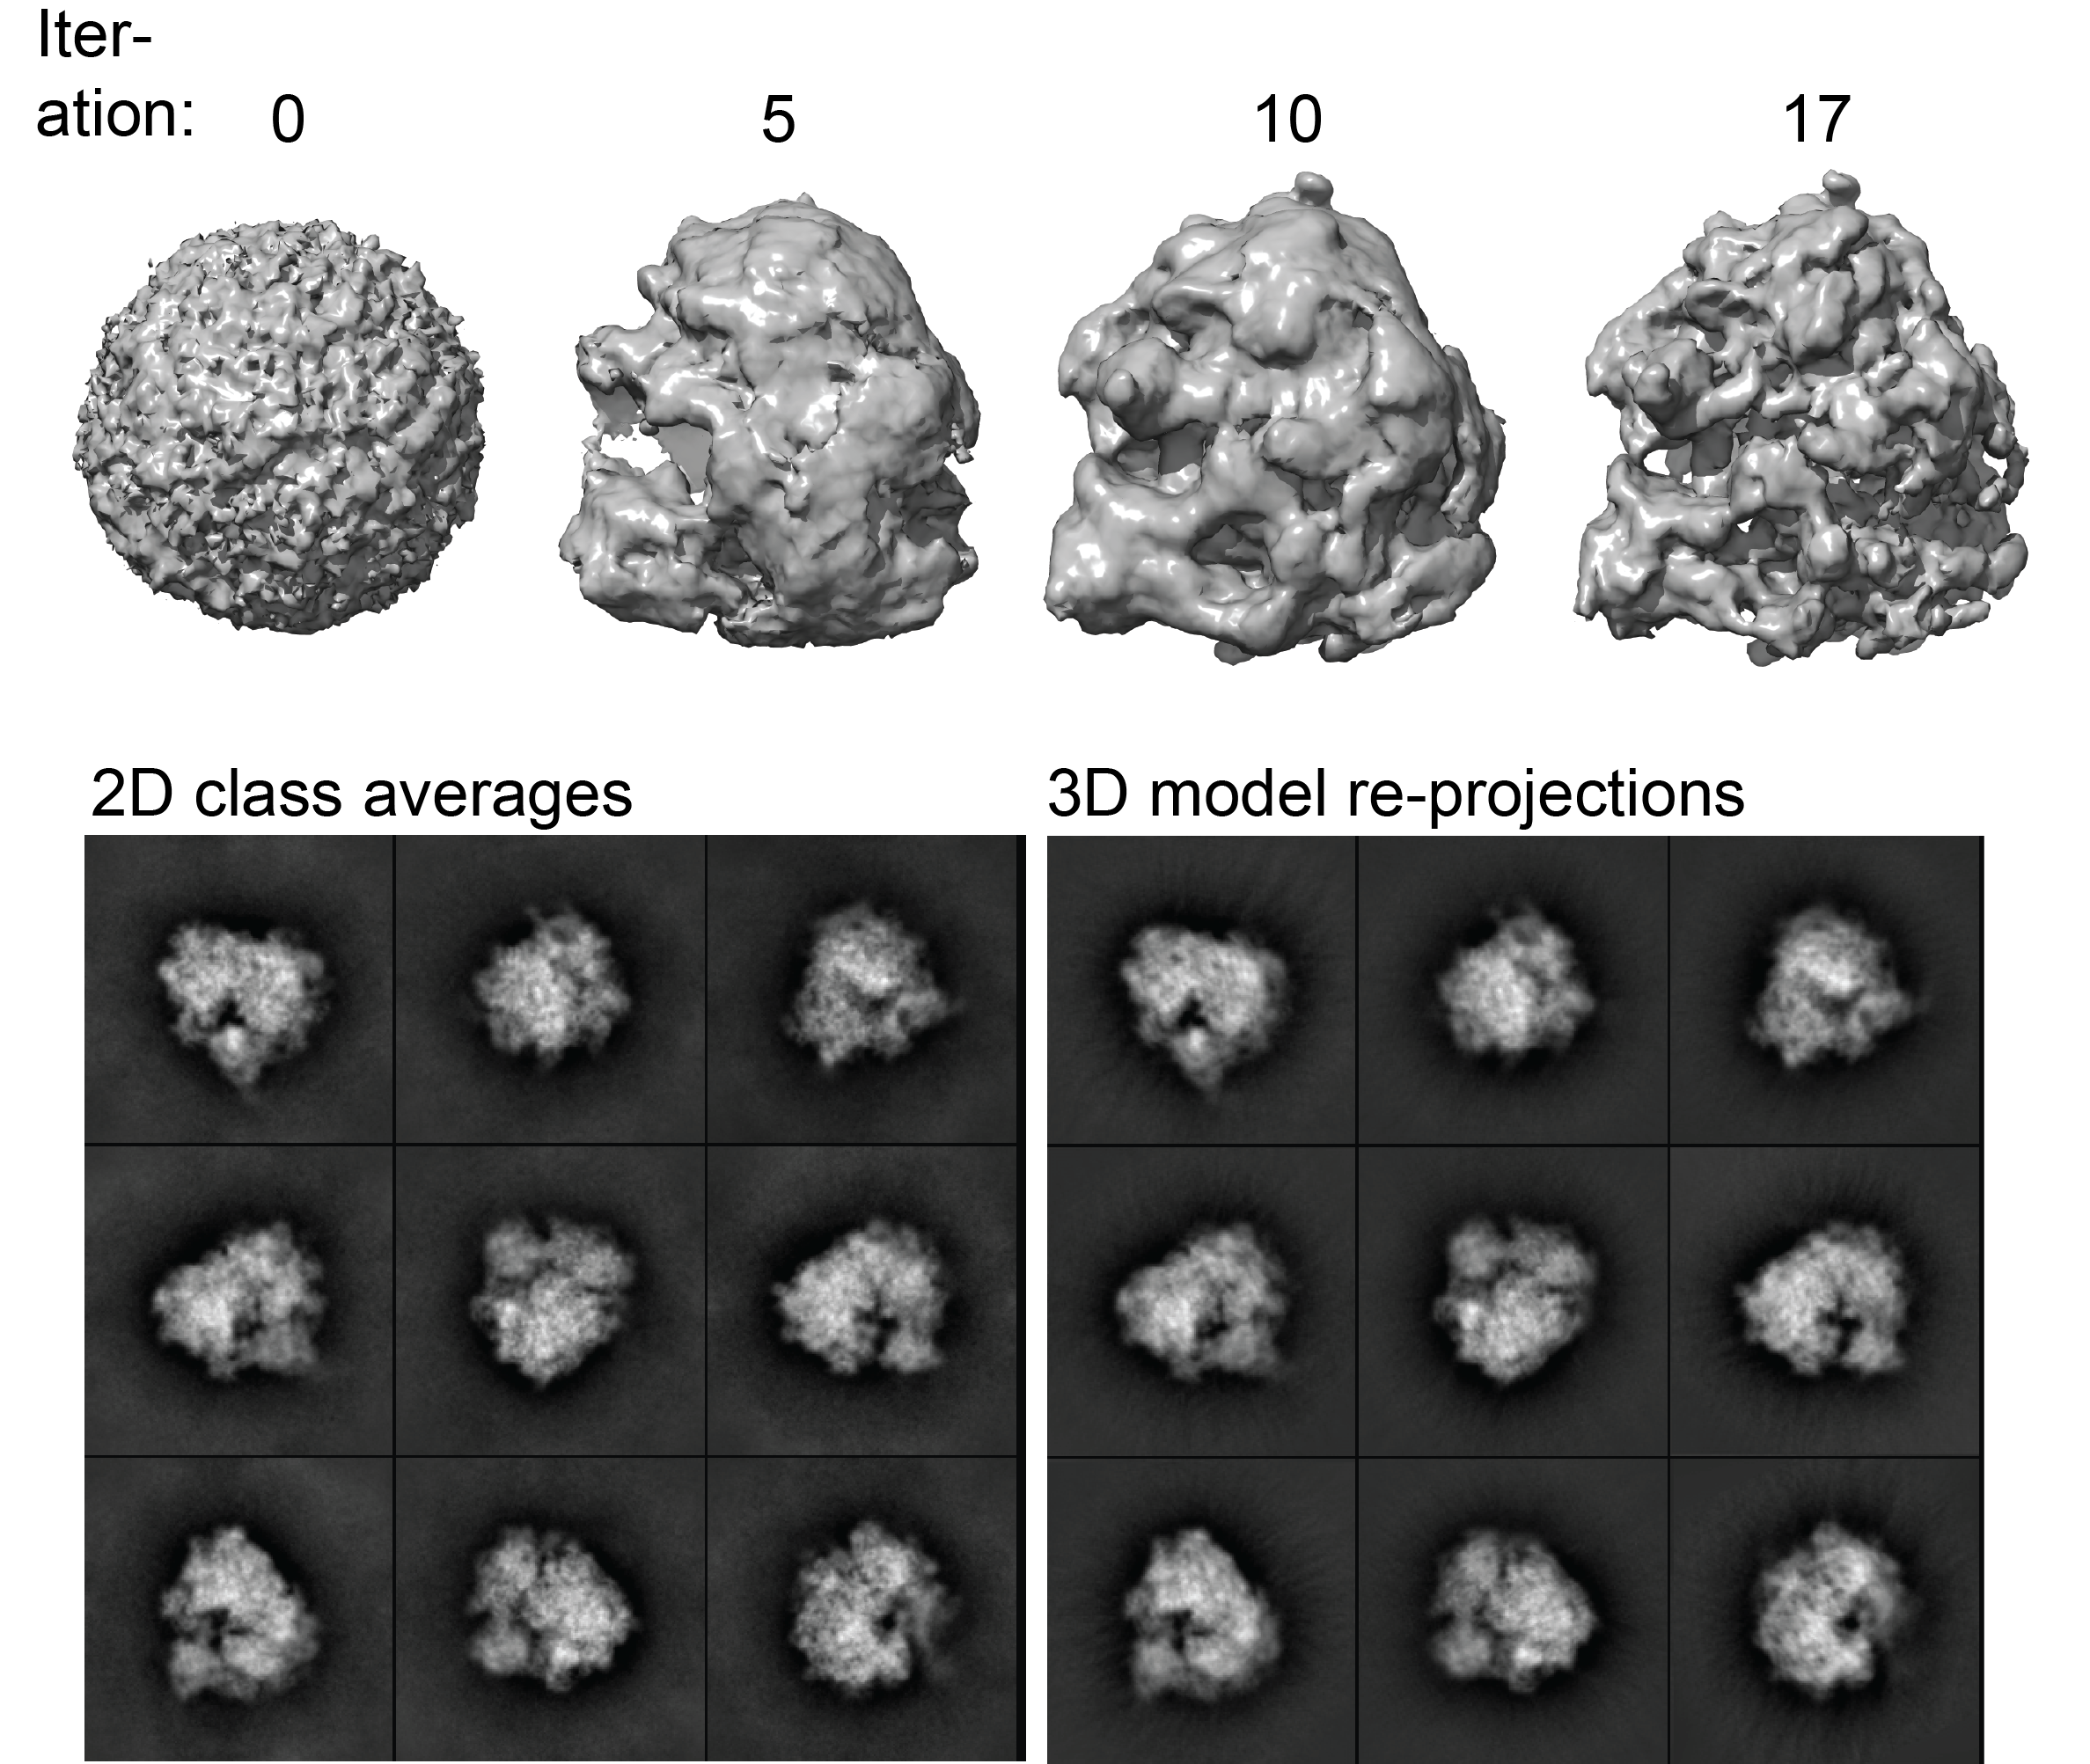
\includegraphics[keepaspectratio=true,scale=0.6]{./Pfrib3D/Pfrib3D}
\caption{Progress of the 3D model throughout the stochastic PRIME3D search (top). Class averages vs. re-projections of the converged 3D reconstruction (bottom).}
\end{figure}
The overlap parameters are very similar to those in \prgname{prime2D} but the \texttt{CLASS DISTRIBUTION OVERLAP} now corresponds to projection directions rather than 2D classes. New statistics include \texttt{AVERAGE ANGULAR DISTANCE BTW ORIS}, which is the average angular distance (in degrees) between the present and the previous sets of best orientations. Since every particle image is assigned a distribution of orientations with associated weight factors, there is also an estimate of the angular standard deviation of the model \texttt{ANGULAR SDEV OF MODEL}. For asymmetric molecules, we expect the angular standard deviation to decrease as the procedure approaches convergence. However, if we reconstruct symmetric molecules with \texttt{pgrp=c1} or asymmetric molecules with pseudo symmetries, the angular standard deviation may increase with the number of iterations as the orientations become randomly  distributed over the symmetry related configurations. Please, use UCSF Chimera to view the reconstructed density (icon on desktop). The \texttt{*pproc*} output is the post-processed volume (for initial model generation this is simply the volume low-pass filtered with the low-pass limit used for alignment).

\begin{tcolorbox}[breakable,colback=white,colframe=orange,width=\dimexpr\textwidth+12mm\relax,enlarge left by=-6mm]
\subsection{Using SIMPLE in the Wild\textemdash{}Mapping Class Orientations and Selection to the Particles}
In a real-life scenario, you would have used a carefully selected set of class averages \texttt{selected.mrc} to obtain your initial 3D model. In order to map this selection and to compose the 3D orientations assigned to the class averages with the 2D orientations/class parameters obtained with \prgname{prime2D} and produce a 3D alignment/selection at the particle level, use \prgname{map2ptcls}. The command is similar to that introduced above. If your converged class averages from \prgname{prime2D} are \texttt{cavgs\_iter021.mrc}, your selected ones are \texttt{selected.mrc}, and your 3D alignment doc is \texttt{prime3Ddoc\_030.txt} then you do the mapping with the command:
\begin{verbatim}
bash-3.2$ simple_exec prg=map2ptcls stk=sumstack.mrc stk2=selected.mrc
stk3=cavgs_iter21.mrc oritab=prime2Ddoc_021.txt oritab2=prime3Ddoc_030.txt nthr=8
\end{verbatim}
creating a file \texttt{mapped\_ptcls\_params.txt} that you can input with flag \texttt{oritab} to \texttt{simple\_distr\_exec prg=recvol} to reconstruct a volume from particle images.
\end{tcolorbox}

\bibliographystyle{elsarticle-harv}
\bibliography{Prime2bibfile}

\end{document}